%
% File naaclhlt2010.tex
%
% Contact: nasmith@cs.cmu.edu

\documentclass[11pt,letterpaper]{article}
\usepackage{naaclhlt2010}
\usepackage{times}
\usepackage{latexsym}
\usepackage{amsmath}
\usepackage{tikz}
\setlength\titlebox{6.5cm}    % Expanding the titlebox

\title{TITLE HERE}

\author{Ben Reis \\
  Johns Hopkins University\\
  3501 Saint Paul st.\\
  Baltimore, MD 21218, USA\\
  {\tt breis3@jhu.edu}
  \And
  Andrew Zhu \\
  Johns Hopkins University \\
  3700 N. Charles St. \\
  Baltimore, MD 21218, USA\\
  {\tt azhu8@jhu.edu}}

\date{}

\begin{document}
\maketitle
\begin{abstract}
General Game Playing (GGP) programs can learn to play any game it is given a description for. In our project, we aim to use these programs to help generate fun and balanced variants of chess. Our system generates descriptions of these variants using the Game Description Language (GDL). By analyzing gameplay results between pairs of GGP players, and by using genetic algorithms to build variants stochastically, our system is able to traverse the search space of chess variants to find one that is hopefully enjoyable.
\end{abstract}

\section{Introduction}
%Intro here - what's the problem?
% talk about GDL, METAGAME, automated game design
Automated game design is a relatively new topic in artificial intelligence
research. %TODO more here

% Discussion of goals re: interesting+balanced games; (read and) cite AGD
% paper(s).
% Some simple discussion of GGP and general game analysis

We focus on chess because it is a good model of a larger genre of positional
strategy games, which are both interesting to humans and easily amenable to
generic analysis, potentially by computers. Principles developed for creating
and balancing variants of chess can then be generalized and expanded to cover
a much wider field of games.

\section{Encoding Chess-Like Games}
Researchers in automated game design are presently focused on short, simple
videogames with few rules. As far as we know, it has been many years since
someone attempted to construct a system for generating chess-like games, and the
only language we could discover for encoding such games is no longer being
maintained.

On the analysis side of things, an extension of Datalog called the Game
Description Language has become the standard language for formally specifying
games in a manner that can be understood by generic computer players. As there
are a number of existing players and masters that make use of GDL, we decided to
use it as well.

% Discussion of Metagame terminology (possibly break into sidebar?)
As discussed in \cite{agd1}, Pell \cite{metagame} did a great deal of work to
define "chess-like" games formally, in his Metagame workbench for general game
players. While we did not use the specification language he defined, his
terminology and mathematical groundwork was quite useful. The key terms used
here are described below.

\begin{description}
   \item [Direction Vector] A direction vector \(\langle x,y \rangle\) is simply
      a vector over the chessboard. \(x\) represents a difference in file and
      \(y\) represents a difference in rank. A positive vector represents a move
      away from white and to white's right. For example, one of a knight's
      possible moves can be described by \(\langle 1,2 \rangle\), and a white
      pawn's standard move is in the direction \(\langle 0,1 \rangle\).
   \item [Symmetry] Pell defines \textit{forward}, \textit{side}, and
      \textit{rotation} symmetries for his vectors. \textit{Forward} and
      \textit{side} symmetries negate the \(y\) and \(x\) values of the vector,
      respectively, while the \textit{rotation} symmetry swaps them.
   \item [Leap] A leap describes a move where intervening squares on the board
      do not matter; only the destination square has any effect on the move's
      legality, and only the destination can be affected.
   \item [Ride] A ride is a series of leaps in a particular direction, sometimes
      with a maximum number of repetitions. All squares between the start and
      the end of a ride must be empty. A pawn's first-turn move is a ride with
      length \(2\).
   \item [Hop] A hop is a ride where some of the squares must be contain a
      piece, possibly of a specific type.
\end{description}
% End Metagame stuff

\section{Search Algorithms}
Genetic algorithms seemed like a good fit with the simulation based strategy that we picked: both genetic algorithms and the simulations involve randomness in their execution. Because our chess variants have different movements rules for individual pieces, we created an encoding of these movement rules. This encoding is then stochastically mutated and recombined with other encodings during the iterations of the algorithm.

We encode each chess variant to be a set of pieces. Because the game players are responsible for actually placing the pieces on the board (see the Implementation section), our encoding only deals with the movement rules of those pieces. Each piece in a variant has a list of movement rules (squares a piece can move into if not capturing a piece) and a list of capture rules (squares a piece can move into if capturing an enemy piece). Each of these rules consists of a direction vector, a ride length, and a list of symmetries that the rule is subject to.

Here are some ways that regular chess pieces would be encoded:\\
\begin{center}
Knight (Figure 1)
\end{center}
\begin{figure}
\centering
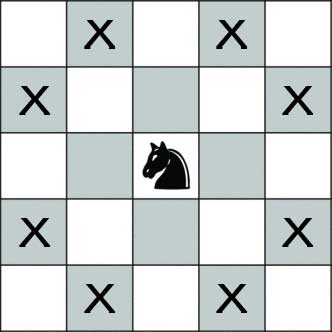
\includegraphics[width=6cm]{knight.jpg}
\caption{Knight Movement}
\label{fig:boat1}
\end{figure}
Movement Rules:
\begin{enumerate}
\item direction:(1,2),\\
rideLength:1,\\
symmetries:[SIDE, FORWARD, DIAGONAL]
\end{enumerate}
Capture Rules:
\begin{enumerate}
\item direction:(1,2),\\
rideLength:1,\\
symmetries:[SIDE, FORWARD, DIAGONAL]
\end{enumerate}

\begin{center}
Queen
\end{center}
Movement Rules:
\begin{enumerate}
\item direction:(1,0),\\
rideLength:7,\\
symmetries:[SIDE, DIAGONAL]
\end{enumerate}
Capture Rules:
\begin{enumerate}
\item direction:(1,1),\\
rideLength:7,\\
symmetries:[SIDE, DIAGONAL]
\end{enumerate}

Recall that diagonal symmetry is symmetry over the $y=x$ axis. This was renamed from Pell's rotational symmetry. This allows the knight movement rule to be encoded simply as one move with all 3 kinds of symmetry. Also recall that a ride is defined as consective movements where no intervening square is occupied, except for perhaps the last square on a capture move. The queen can traverse the entire board if not blocked, so she has a ride length of 7 to represent 7 consecutive movements in the direction (1,0) or (1,1). Both of the examples here have the same rules for capture and movement. A pawn would have two different rules in order to encode that a pawn can move forward if not blocked by another piece, and can only capture diagonally. Every piece in our encodings has side symmetry (across the $y$ axis) for aesthetic reasons.

When running the algorithm, there are $N$ surviving variants after a round of selection. During the generation phase, we generate an additional $N$ candidate variants for the next round using mutation and recombination. A candidate is mutated by adding new pieces to its set of pieces, by deleting pieces, or by changing the movement rules of its existing pieces. Two candidates are recombined into a new candidate by picking randomly among the two parents' pieces to create a new set of pieces. The original $N$ variants also remain in the pool of survivors, unchanged.

After the generation phase comes the selection phase, where candidates are evaluated using the GGP players, and then some candidates are thrown out before the next generation phase. In keeping with the spirit of games, we decided to use tournament selection to select $N$ survivors from the $2N$ candidates. A fitness score is calculated for each candidate based on the results from the GGP players, and then candidates are randomly paired with each other. The candidate with the higher fitness score in each pair is selected to survive. Note that in this scheme, the candidate with the best fitness score will always survive, and candidates with higher scores are more likely to survive, but not guaranteed.

Fitness values are calculated based on statistics collected by the GGP players. To keep games fair, we would like the win rate to be about $1/2$ for each player, so the fitness value is calculated based on deviation from this win rate. We currently use only the win rate of white vs black to determine fitness, but we would like to use other metrics in the future to tailor our results. Incorporating the average length of games would help make sure that games aren't too short or too long. Pieces also should not be too complicated for human users to remember, so pieces with few movement rules should be preferred over those with long lists of rules.

\section{Implementation}
% Decided to have players place pieces to simplify game generation.

\subsection{Generating Pieces}
% talk about balance decisions
% talk about rules we omitted

\subsection{Encoding the Game}
% talk about encoding decisions in GDL
% cite speedchess; alloyGGP
Encoding chess in GDL presents a number of problems due to the complexity of the
game's state, which involves a great deal of information on which pieces have
moved at all (for pawn moves and castling) and which pieces might move to
certain places (for check and related concepts). All of this is in addition to
the \(32\) pieces that may be on the board and the \(64\) cells that make it up.

The work of Alex Landau in writing a slightly trimmed-down version of chess, as
well as his more general work in GDL was invaluable for the code generation
process. The fundamental arithmetic clauses we use are his directly
\cite{gdlmath}, and many other elements of our code is based on his Speedchess
\cite{spdchess} implementation of the game.

Other than a few counters and a phase marker, game state is tracked entirely by
which squares contain pieces. Other cells are essentially "brought into
existence" as they are needed. This greatly reduces the ammount of state that
players and the game master need to handle, but increases the size of the rules,
as capture and non-capture moves must be handled separately.

To reduce the number of games which need to be evaluated, we have players place
pieces themselves, purchasing them from a list that defines the game being
played. In an extra phase before the game begins, players simultaneously place
one piece each, as they choose, anywhere on a number of ranks associated with
the variant they are playing. Each must place exactly one king, and the king
must be placed last. There are no pawns unless the piece generation algorithm
produces them. Once both players have placed their king, the game begins.

To simplify both the GDL code generation process and the resulting output, we
have chosen to omit moves whose legality depends on facts other than the current
state of the board. We also ignore the notion of check; players are instead
required to capture the enemy king. Since GDL requires that games be finite in
length, we force a draw after a number of moves, as is common in implementations
of boardgames which can draw.

\subsection{Running the players}
We used the GGP server from GGP.org to host our games. This server sends data over a network using HTTP requests to communicate with the players. Our GGP Player was the award winning CadiaPlayer, which uses refined Monte Carlo tree search methods to make gameplay decisions. After the server is connected to its two players, it sends the game description and game state to each player, and gives the active player a limited amount of time (15 seconds) to respond with a valid move. Gameplay continues in this fashion until a terminal state is reached. Our program is capable of starting up multiple instances of the server and multiple players to speed up the running time.

\section{Results}
We were not able to run the code on chess variants because we were not able to work out all the bugs with generating the GDL code from an encoding. However, we were able to execute some benchmarks that give some idea about how the solver will perform if our system was fully functional. We also were able to test most parts of the system individually to make sure that they run according to the specification.

Before testing with chess variants, we tested the players with Tic-Tac-Toe, which is a very simple game with a decision tree that can be constructed very easily. As expected, the CadiaPlayer solvers are able to play this game optimally, and always ends the game in a draw when facing against itself. However, the CadiaPlayer still takes all the time it is given before making a decision. It is therefore critical to choose an appropriate amount of time for a given game in order to speed up computation so that gameplay doesn't hang while the CadiaPlayer is already finished, or while it traversing very deep levels of the decision tree with no real hope of learning much more. The players were still able to play optimally when given only 3 seconds to respond with a move in Tic-Tac-Toe.

We tested the solver on harder games like connect four and chess. The solver was able to play connect four competitively, but was not very competent at chess, and seemed to make somewhat random movements. This is likely due to the large branching factor of chess, since there are so many moves to consider. Connect four is somewhat complex, but because there are only up to 8 possible moves to consider in any given state, so the decision tree is still manageable. We were aware of the large branching factor of chess from the start of our project, and we decided to stick with smaller boards with a few pieces on each side to lessen the problem.

We also extensively tested the genetic algorithm's generation phase, making sure that it creates valid variants. We chose probabilities for each type of mutation (adding/deleting pieces, adding/deleting moves of pieces, changing movement vectors and symmetries) to make sure mutations were not too drastic.

\section{Discussion}
% stuff on costs -> incorporating it into the games? better calculation
% stuff on redundancy of encodings

\section{Comparison to Proposal}


\section{Future Work}
% how to test! -> start small, work up

\subsection{Evaluating Games}

\subsection{Improving Performance}

Almost all of our runtime is spent processing GDL through Cadia and the GGP
server. Aside from bug fixes, the first obvious performance improvement to be
made in this area would be the addition of \textit{base} and \textit{input}
clauses to our generated code. These are optional (and somewhat nonstandard)
clauses that many players use to speed up their analysis of games by never
considering illegal moves or impossible game states.

\subsection{Features Omitted}

As discussed above, we omitted a number of features defined in \cite{metagame},
and features that might be considered "typical" in chess variants.

Most obviously, our current generator does not (and cannot) produce the standard
"front rank" of pawns that appears in most versions of chess. Adding this in as
an element that the generator could choose to add to a game would be fairly
straightforward.

Our code currently lacks three major features of Metagame: leaps, promotions,
and drops. Leaps, as stated above, are a movement option. A promotion is a rule
by which a piece can change its type, usually upon reaching the opponent's back
rank. Both of these would complicate the piece generator, since their mechanics
and their value depend on the existence and value of other pieces. Pawn
promotions, as in chess, would be very easy to implement, though; it would be a
simple change to the generated GDL for pawns, once such was added. Drops are
another more complicated thing to add, this time to the GDL. A drop is a move
where one player adds a piece (usually one they have captured) to the board that
was not there before. Adding drops would require that the GDL code track which
pieces a player has captured, and which they have dropped. This would not be too
difficult, since captures are already slightly separated from regular moves, but
it would be nontrivial.

Metagame also allows for variation in the players' goal; this would be more or
less straightforward to add to the game, depending on what alternate goals are
allowed and what effects these alternate goals have on piece placement rules. If
desired, different goals could be scored differently, allowing players to aim
for alternate objectives if their primary goal is not likely to be achieved.

\section{Conclusion}
% reiterate approach, findings
\printbibliography

\end{document}
